\newcommand{\titel}{Report for ARM Microcontroller Project}
\title{\titel}
\newcommand{\untertitel}{uLoader WiSe 2014}
%\subtitle{\untertitel}
\newcommand{\autor}{Appel, Dennis (s813783)\\Voigt, Alexander (s814526)\\Merrikhi, Pedram (s827711)}
\author{\autor}
\date{\today}

\documentclass[
	11pt,				% Schriftgröße
	DIV10,
	english,         		% für Umlaute, Silbentrennung etc.
	a4paper,			% Papierformat
	oneside,			% einseitiges Dokument
	titlepage,			% es wird eine Titelseite verwendet
	parskip=half,			% Abstand zwischen Absätzen (halbe Zeile)
	headings=normal,		% Größe der Überschriften verkleinern
	listof=totoc,			% Verzeichnisse im Inhaltsverzeichnis aufführen
	bibliography=totoc,		% Literaturverzeichnis im Inhaltsverzeichnis aufführen
	index=totoc,			% Index im Inhaltsverzeichnis aufführen
	captions=tableheading,		% Beschriftung von Tabellen unterhalb ausgeben
	final,				% Status des Dokuments (final/draft)
	numbers=endperiod
]{scrreprt}

\usepackage{float}
\restylefloat{table}

\usepackage{scrhack}
\usepackage{yfonts}
% Zum Umfließen von Bildern -------------------------------------------------
\usepackage{floatflt}
\usepackage{lmodern}
\usepackage{textcomp}			% Euro-Zeichen etc.
\usepackage{color}
\usepackage{listings}

\definecolor{codegreen}{rgb}{0,0.6,0}
\definecolor{codegray}{rgb}{0.5,0.5,0.5}
\definecolor{codepurple}{rgb}{0.58,0,0.82}
\definecolor{backcolour}{rgb}{0.95,0.95,0.92}

\lstset{ %
	backgroundcolor=\color{backcolour},
	commentstyle=\color{codegreen},
	keywordstyle=\color{magenta},
	numberstyle=\tiny\color{codegray},
	stringstyle=\color{codepurple},
	basicstyle=\footnotesize,
	breakatwhitespace=false,
	breaklines=true,
	captionpos=b,
	keepspaces=true,
	numbers=left,
	numbersep=5pt,
	showspaces=false,
	showstringspaces=false,
	showtabs=false,
	tabsize=2
}
\usepackage[english]{babel}		% neue deutsche Rechtschreibung
\usepackage[utf8]{inputenc}
\usepackage[T1]{fontenc}
\usepackage{url}			% URL-Highlighting
\usepackage{amsmath,amsfonts}
% \usepackage{amsmath}
%\usepackage{times}
\usepackage{setspace}
\usepackage{multirow}
%\usepackage{amsfonts}
%\usepackage{amssymb}
\usepackage{array}
\usepackage[
	automark,			% Kapitelangaben in Kopfzeile automatisch erstellen
	headsepline,			% Trennlinie unter Kopfzeile
	ilines				% Trennlinie linksbündig ausrichten
]{scrpage2}
\usepackage[labelfont=bf, belowskip=4pt, hypcap]{caption}
\usepackage{a4wide}
\usepackage[acronym,toc]{glossaries}
%\usepackage{mathrsfs}
%\usepackage{mathtools}
\usepackage{graphicx}
%\usepackage{wasysym}
%\usepackage{pgfplots}
\usepackage{cite}
% Text um Bilder fliessen lassen
\usepackage{wrapfig}
\usepackage{float}
\usepackage{pdfpages}
\usepackage{geometry}
% \geometry{paper=a4paper,left=35mm,right=35mm,top=30mm}
\usepackage[square]{natbib}
\usepackage{tikz}
\usetikzlibrary{arrows,shapes,positioning,shadows,trees}

\tikzset{
  basic/.style  = {draw, text width=2cm, drop shadow, font=\sffamily, rectangle},
  root/.style   = {basic, rounded corners=2pt, thin, align=center,
                   fill=green!30},
  level 2/.style = {basic, rounded corners=6pt, thin,align=center, fill=green!60,
                   text width=8em},
  level 3/.style = {basic, thin, align=left, fill=pink!60, text width=8em}
}

% Kopf- und Fußzeilen
\pagestyle{scrheadings}

% Kopf- und Fußzeile auch auf Kapitelanfangsseiten
\renewcommand*{\chapterpagestyle}{scrheadings}

% Schriftform der Kopfzeile
\renewcommand{\headfont}{
	\normalfont
}

% Kopfzeile
\ihead{\large{\textsc{\titel}}\\ \textit{\headmark}}
\chead{}
\ohead{} %\vspace{0.5cm} \includegraphics[scale=0.3]{Beuth_Logo_horizontal}}
%
\setlength{\headheight}{21mm}		% Höhe der Kopfzeile
\setlength{\parindent}{5mm}		% Einzug bei neuem Absatz
\setheadwidth[0pt]{textwithmarginpar}	% Kopfzeile über den Text hinaus verbreitern
\setheadsepline[text]{0.4pt}		% Trennlinie unter Kopfzeile

% Fußzeile
\ifoot{}
\cfoot{\textsc{\footnotesize{\untertitel}}}
\ofoot{\pagemark}

\subtitle{\untertitel}

% erzeugt ein wenig mehr Platz hinter einem Punkt
\frenchspacing

% Schusterjungen und Hurenkinder vermeiden
\clubpenalty		= 10000
\widowpenalty		= 10000
\displaywidowpenalty	= 10000

% mach pdf searchable
\usepackage{lmodern}
\input{glyphtounicode}
\pdfgentounicode=1

% \usepackage[bookmarks,bookmarksnumbered]{hyperref}
\usepackage[
bookmarks,
bookmarksopen=true,
pdftitle={\titel},
% pdfauthor={\autor},
% pdfcreator={\autor},
pdfsubject={\titel},
pdfkeywords={\titel},
colorlinks=true,
linkcolor=red, % einfache interne Verknüpfungen
anchorcolor=black,% Ankertext
citecolor=blue, % Verweise auf Literaturverzeichniseinträge im Text
filecolor=magenta, % Verknüpfungen, die lokale Dateien öffnen
menucolor=red, % Acrobat-Menüpunkte
urlcolor=cyan,
% linkcolor=black, % einfache interne Verknüpfungen
% anchorcolor=black,% Ankertext
% citecolor=black, % Verweise auf Literaturverzeichniseinträge im Text
% filecolor=black, % Verknüpfungen, die lokale Dateien öffnen
% menucolor=black, % Acrobat-Menüpunkte
% urlcolor=black,
backref,
%pagebackref,
plainpages=false,% zur korrekten Erstellung der Bookmarks
pdfpagelabels,% zur korrekten Erstellung der Bookmarks
hypertexnames=false,% zur korrekten Erstellung der Bookmarks
% linktocpage, % Seitenzahlen anstatt Text im Inhaltsverzeichnis verlinken
% linkcolor=red % Linkfarbe f\"ur den Druck auf schwarz, f\"ur die PDF-Version auf rot stellen
]{hyperref}

\setcounter{secnumdepth}{5}
\setcounter{tocdepth}{5}
\newcommand*{\fullref}[1]{\hyperref[{#1}]{\autoref*{#1} \nameref*{#1}}}

\makeindex
\makeglossaries

\begin{document}
\maketitle
\pagenumbering{Roman}
\tableofcontents
\newglossaryentry{can}{name=CAN, description={Controller Area Network ist ein serrieller BUS der asynchron arbeitet. 1 Mbit/s ist hierbei die Maximale Datenrate. Wird meist in Fahrzeugen eingesetzt. }}
\newglossaryentry{ahb1}{name=AHB1, description={Advanced High-performance Bus is part of the Advanced Microcontroller Bus Architecture (AMBA) of the IP-manufacturer ARM Limited (ARM).}}
\newglossaryentry{apb}{name=APB, description={The Advanced Peripheral Bus (APB)
 is an internal bus for System-on-Chips (SoC) to connect low power peripheral
 devices. The APB bus is part of the AMBA-achitecture which is designed for low
power and simple interface. It can be used with the standardized buses like AHB.}}

\newglossaryentry{SWD}{name=SWD, description={Serial Wire Debug is an alternative 2-pin electrical interface that uses the same protocol. It uses the existing GND connection. SWD uses an ARM CPU standard bi-directional wire protocol, defined in the ARM Debug Interface v5.}}

\newglossaryentry{MCU}{name=MCU, description={Microcontroller Unit is a small computer on a single integrated circuit containing a processor core, memory, and programmable input/output peripherals. Program memory in the form of Ferroelectric RAM, NOR flash or OTP ROM is also often included on chip, as well as a typically small amount of RAM.}}

\newglossaryentry{LVM}{name=LVM, description={Logical Volume Manage provides a method of allocating space on mass-storage devices that is more flexible than conventional partitioning schemes. In particular, a volume manager can concatenate, stripe together or otherwise combine partitions (or block devices in general) into larger virtual ones that administrators can re-size or move, potentially without interrupting system use.}}

\newglossaryentry{ROM}{name=ROM, description={Read Only Memory is a class of storage medium used in computers and other electronic devices.}}

\newglossaryentry{USB}{name=USB, description={Universal Serial Bus is an industry standard developed in the mid-1990s that defines the cables, connectors and communications protocols used in a bus for connection, communication, and power supply between computers and electronic devices.}} 

\newglossaryentry{UART}{name=UART, description={universal asynchronous receiver/transmitter is a piece of computer hardware that translates data between parallel and serial forms. UARTs are commonly used in conjunction with communication standards such as EIA, RS-232, RS-422 or RS-485. The universal designation indicates that the data format and transmission speeds are configurable.}}

\newglossaryentry{JTAG}{name=JTAG, description={Joint Test Action Group was formed in 1985 to develop a method of testing finished printed circuit boards after manufacture. In 1990, the effort was codified as a standard by the Institute of Electrical and Electronics Engineers with the designation IEEE Std. 1149.1-1990 entitled Standard Test Access Port and Boundary-Scan Architecture.}}

\newglossaryentry{AMBA}{name=AMBA, description={Advanced Microcontroller Bus Architecture is an open-standard, on-chip interconnect specification for the connection and management of functional blocks in system-on-a-chip (SoC) designs. It facilitates development of multi-processor designs with large numbers of controllers and peripherals.}}

\newglossaryentry{CMSIS}{name=CMSIS, description={Microcontroller Software Interface Standard, is a vendor-independent hardware abstraction layer for the Cortex-M processor series and specifies debugger interfaces.}}

\newglossaryentry{AHB}{name=AHB, description={AHB, please refer to AMBA}}

\newglossaryentry{NVIC}{name=NVIC, description={Nested Vectored Interrupt Controller,facilitates low-latency exception and interrupt handling, controls power management, implements System Control Registers. The NVIC supports up to 240 dynamically reprioritizable interrupts each with up to 256 levels of priority.}}

\newglossaryentry{GPIO}{name=GPIO, description={General-purpose input/output is a generic pin on an integrated circuit whose behavior, including whether it is an input or output pin, can be controlled by the user at run time}}

\newglossaryentry{USART}{name=USART, description={universal synchronous/asynchronous receiver/transmitter, modern ICs now come with a UART that can also communicate synchronously}}

\newacronym{RCC}{RCC}{Reset and Clock Control}
\newacronym{TAP}{TAP}{test access ports}
\newacronym{AHB}{AHB}{Advanced High Performance Bus}

% \hypertarget{glossar}{\printnomenclature}
\label{sec:Glossar}
\printglossaries
\listoffigures					% Abbildungsverzeichnis
\listoftables					% Tabellenverzeichnis
\lstlistoflistings
\clearpage
\pagenumbering{arabic}
\chapter{Introduction}
 
Nowadays, an ARM-MCU could be used in every aspect of everyday life.
Additionally, the ARM processor is the number one architecture of choice in 
many market segments.\\\\ 
This project is based on the development of a bootloaders and its implementation 
inside a network. The usage stm32f4-discovery Board is a prefered and viewed as an 
"'Allrounder"' for such a project. The reasoning behind this is the "value for money" 
and user-friendliness. This allows for an easy introduction into the world of ARM
Microcontroller unit programming.\\
The ARM-Cortex-M4-Prozessor found on the STM32f4-discovery board processes 
the principel parts shown in the figure below.\\
The aim of the project is to research the feasibility to create a quick, cheap 
and easy to use way of utilizing an STM32 Microcontroller to communicate between 
a user and a remote device.\\\\
The purpose of the application is meant to be a first step fundamental strategy to 
creating a product for future projects.\\
It is hoped that by utilizing a boot loader, a fast and light application could 
be used to fulfill the desire of a user to achieve a particular objective such 
as, threeway handshake signal to verify a particular device in order to transmit 
information such as codes or messages, using a TCP/IP protocol stake.\\
As it can be demonstrated the different applications could be endless.\\ 

\begin{figure}[ht]
	\centering
	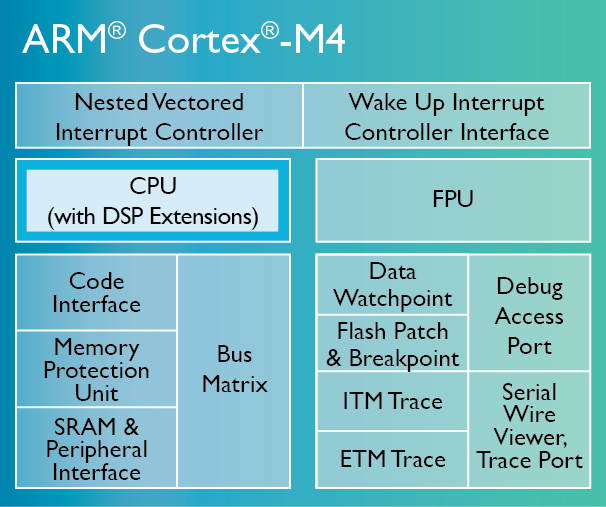
\includegraphics[width=400px, height=300px]{../img/Cortex-M4-chip-diagram-LG.png}
	\caption{Prinzipieller Aufbau}
	\label{m4_prinzip}
\end{figure}

Analogously, a new and different diagram would be used, in order to illustrate the 
change in the usage-concept of the processors.\\

But first, an overview of the discussed focal points would be outlined.\\  


\section{Bootloader}
The purpose of a Bootloader program is to allow the installation and utilisation 
of any program that could be reloaded. Whereas the program that is currently loaded is also being run.\\
Next it is necessary to initialise the hardware, that would in turn be needed to load the program.\\
The "STM32f407 discovery board" offers three different methodes to boot up the hardware.\\
In order to switch between the three different boot methods, the Boot-Pins BOOT1
and BOOT2 could be set:
\begin{table}[ht]
\centering
\begin{tabular}{|c|c|l|l|}
\hline \hline
  BOOT1 & BOOT2 & Boot-Mode & Adresse\\ \hline
  x & 0 & Flash Memory (User Flash) & 0x8000\_0000\\
\hline
  0 & 1 & System Memory & 0x1FFF\_F000\\
\hline
 1  & 1 & SRAM & 0x2000\_0000\\
\hline
\end{tabular}
\caption{Boot-Pin Function}
\end{table}\\\\

The ROM memory is included by the manufacturer along with the bootloader.\\
It is very important to set the correct address of the program, that is located 
in the memory, in order for the reloading of the program to work.\\
A step by step example of the the sequence after the boot loader is already 
loaded , is as follows:

\begin{enumerate}
\item Hardware initialize (USB / USART / RCC ... )
\item Wait for running program (pending other tasks)
\item Write a program to address XY.
\item Point to address XY
\end{enumerate}

After these steps, the newly setup program is then responsible for the initialization 
of the hardware.\\

\section{SWD}
During the development of the Boot Loader, a serial wire debug technology was used. 
The reason behind this is to utilize a Debug-Port that has been specially developed to 
cater to a MCU that makes allows the use of the least amount of pins possible.\\
This port consists of pins shown in the following:\\
\begin{table}[ht]
\centering
\begin{tabular}{|c|c|c|p{10cm}|}
\hline \hline
	Pin & Signal & Type & Description \\ \hline
1 & VTref & Input & This is the target reference voltage. It is used to
 check if the target has power, to create the logic-level reference for
 the input comparators and to control the output logic levels to the target.
 It is normally fed from Vdd of the target board and must not have a series resistor.\\ \hline
7 & SWDIO & I/O & Single bi-directional data pin\\ \hline
9 & SWCLK & Output & Clock signal to target CPU. It is recommended that
 this pin is pulled to a defined state of the target board. Typically
 connected to TCK of target CPU.\\ \hline
13 & SWO & Output & Serial Wire Output trace port. (Optional, not required
for SWD communication)\\ \hline
15 & RESET & I/O & Target CPU reset signal. Typically connected to the
 RESET pin of the target CPU, which is typically called "nRST", "nRESET"
 or "RESET".\\ \hline
19 & 5V-Supply & Output & This pin is used to supply power to some eval boards.
Not all JLinks supply power on this pin, only the KS (Kickstart) versions.
Typically left open on target hardware.\\ \hline
\end{tabular}
\caption{SWD PINOUT}
\end{table}\\

The other pins of the 20-pole connection are going to left out, meaning, the other 
pins are useless for the SWD or they will be used as a GND. Regardless of the pin allocation, 
it is important that the communication of the SWD would not be interrupted or effected. 

This technique represents a new and more effective way to debuggen. Until now JTAG 
represented the Debugger-Interface.  


The advantages of this technology are:

\begin{itemize}
\item Only 2 Pins are used
\item JTAG TAP controller compatible
\item Allows the Debugger to become an extra AMBA-Bus-Master, in order to accomidate an extra 
access capability to the Register or Memory
\item High Datarates - 4Mbytes/sec @50MHz
\item Low Power - no extra power supply 
\item Error recognition "'built in"' that performs well
\item Protection against errors that cause disconnection
\end{itemize}  

\section{Startup}
 - stack, program counter, interrupt, vector table, initial system clock

\section{CMSIS}
The ARM Cortex Microcontroller Software Interface Standard is a manufacturer independent 
abstraction layer for the Cortex-M processors.\\
Thereby the CMSIS is subdivided into:
\begin{itemize}
\item CMSIS-CORE - API access to the processor kernal and peripheral register.
\item CMSIS-Driver - Generic access on peripheral devices for Middleware
			(reusability).
\item CMSIS-DSP - DSP Liberary with over 60 functions
\item CMSIS-RTOS API - Standardised (RTOS compatible)
\item CMSIS-Pack - Description of the most important components (User view)
\item CMSIS-SVD - Description of the most important components (System view)
\item CMSIS-DAP - Debug Access Port
\end{itemize}

Summarized, CMSIS allows a consistent and simple software interfaced to the processor 
and peripheral devices, as well as Real-time OS (RTOS) and Middleware.

\section{Nested Vectored Interrupt Controller}
The NVIC offers the possibility to configure special interrupts 
(Priority, Activate, Deactivate...). \\
Aside from the given interrupts, there are also the configurable implementation dependent interrupts.  
Because, the first 15 interrupts are allocated, the number of implimented interrupts could be from 0-240.

\section{Differences }
GNU, KEIL iar

\section{Network}
was sollte zum besseren verstehen hier einen platz finden.

\chapter{ARM M4}
The ARM M4 MCU is the heart of the stm32f407. ARM offers the IP of the
CORE-M4 to manufacturers and they can customize the IP as they see fit.
A very simple diagram of the used MCU is the following:\\

\begin{figure}[ht]
	\centering
	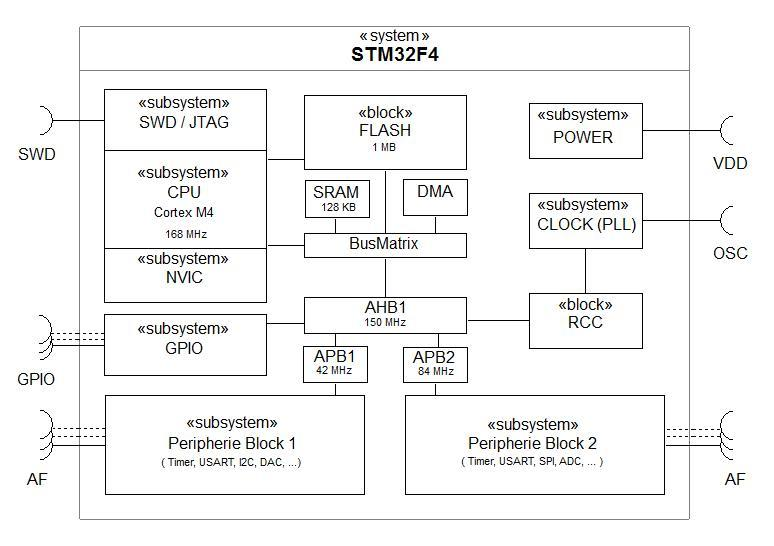
\includegraphics[width=400px,height=300px]{../img/stm32f4_prinzip.jpeg}
	\caption{Simple M4 Diagram}
	\label{m4_simple}
\end{figure}

The diagram doesn't show, which peripheral systems are connected to which
APBX-Bus, but that can be seen in the datasheet. What it does show is, that
the GPIO-Pins, are connected to the AHB1-Bus.\\
The reason for that is, that it's much faster then what is recommended
 for most the part of what a GPIO demands. The subsystems on the other hand aren't
 necessarily needed to react that fast.\\

For example the USART6, which is used in the project, is connected to APB2.
A much more precise representation of the STM32F4 is illustrated in the following diagram.\\

The AHB1 is the system bus and therefore should be really fast.
\includepdf[pages={18}]{../img/blockdia.pdf}

The peripheral systems are addressed through the busses. For example the
GPIOA and USART6.
The address range of the peripherals is 0x4000\_0000 - 0x5FFF\_FFFF. The
peripheral base address is 0x4000\_0000. To configure and write to / read from
the USART6 we need the peripheral base address and an offset. In the case of
USART6 the offset is a combination of two offsets, as seen in the table:
\includepdf[pages=73]{../img/blockdia.pdf}
\begin{enumerate}
	\item Peripheral Base: 0x40000000
	\item APB2: Peripheral Base + 0x10000 = 0x40010000
	\item USART6\_Base: APB2 + 0x1400 = 0x40011400
\end{enumerate}

At the USART6\_Base is equal to the USART Status register. To transceive data
via USART6 the DR register (16-bit) with an additional offset of 0x04 is right
one.

It is one register to read to and write from. That is a good example, why an
interrupt handler is needed (NVIC). The program would have a huge timing problem
since the read operation on that register would cause a huge delay, because
it would wait till data is read.

On this way all the peripherals are can be addressed.
For the GPIOA it is theoretically the same but with other addresses. The GPIOA
is connected via the faster AHB1 bus.
\begin{enumerate}
	\item AHB1\_Base: Peripheral Base + 0x20000
	\item GPIOA\_Base: AHB1\_Base
\end{enumerate}
These are just two examples of the addressing of the ARM peripherals, but at the
bottom they are all the same - it's all about the addresses.

\chapter{NVIC in use}
As already mentioned, the NVIC is used to configure the interrupts. Since
there is a bi-directional communication via USART6, the NVIC has to be
configured to fit that demand.\\
Therefore the first thing to do is to enable the clock on APB2 to clock
the USART6. Additionally configuration has to be done for the USARTX,
 but it is not part of the NVIC configuration.\\
The clock is mentioned because it plays an essential part of the configuration.
It is not important which U(S)ART[1..6] pin is used. Naturally, the right APBX
has to be configured (precise diagram of stm32f4).

The configuration is done by writing the parameters into a structure and
binding them and than load it into the NVIC.
The last thing to do is to enable USART globally.

\begin{lstlisting}[language=C,caption={enable usart},label=lst:usart]%[ht]
/* We are initialized */
u->Initialized = 1;

/* Disable if not already */
USARTx->CR1 &= ~USART_CR1_UE;

/* Init */
USART_Init(USARTx, &USART_InitStruct);

/* Enable RX interrupt */
USARTx->CR1 |= USART_CR1_RXNEIE;

/* Fill NVIC settings */
NVIC_InitStruct.NVIC_IRQChannelCmd = ENABLE;
NVIC_InitStruct.NVIC_IRQChannelPreemptionPriority = TM_USART_NVIC_PRIORITY;
NVIC_InitStruct.NVIC_IRQChannelSubPriority = TM_USART_INT_GetSubPriority(USARTx);
NVIC_Init(&NVIC_InitStruct);

/* Enable USART peripheral */
USARTx->CR1 |= USART_CR1_UE;
\end{lstlisting}

The code is part of a function therefor USARTx is a parameter, in this case it
is USART6.

The process and as well as the code that was used, generated the desired results
 which proves the method that was chosen works.



\chapter{Network}
The Network on the Baseboard is realized through a SMSC LAN8720.

4-bit data nibbles are sent to the MII block. These data nibbles are clocked
to the controller at a rate of 25MHz. The controller samples the data on the
rising edge of RXCLK. To ensure that the setup and hold requirements are met,
the nibbles are clocked out of the transceiver on the falling edge of RXCLK.
RXCLK is the 25MHz output clock for the MII bus. It is recovered from the received
data to clock the RXD bus. If there is no received signal, it is derived from
system reference clock(XTAL1/CLKIN).

When tracking the received data, RXCLK has a miximum jitter of 0.8ns (provided
that the jitter of the input clock, XTAL1/CLKIN, is below 100ps).

In RMII mode, the 2-bit data nibbles are sent to the RMII block. These data nibbles
are clocked to the controller at a rate of 50MHz. The controller samples the data
on the rising edge of XTAL1/CLKIN (REF\_CLK). To ensure that the setup and hold
requirements are met, the nibbles are clocked out of the transceiver on the falling
edge of XTAL1/CLKIN (REF\_CLK).

The blockdiagram \ref{stm32f4_phy} shows the hardware for the RMII for
a network connection.

\begin{figure}[h!]
	\centering
	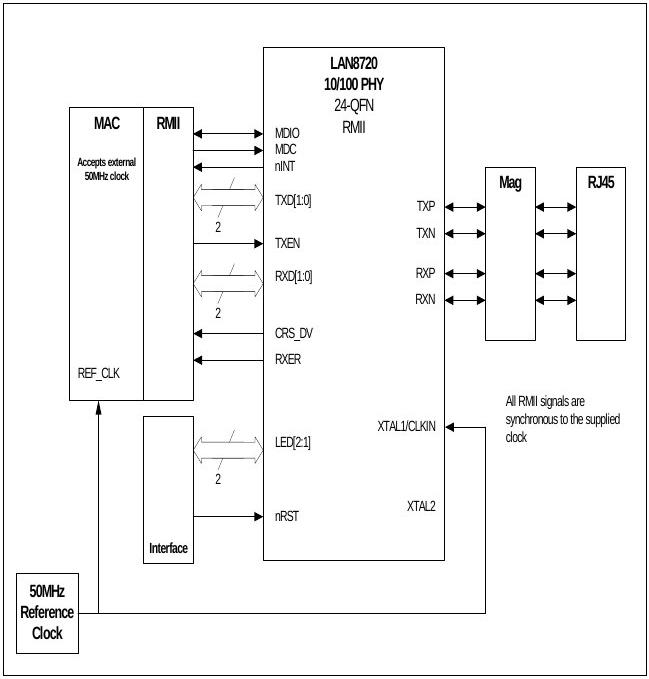
\includegraphics[totalheight=0.36\textheight]{../img/network.jpeg}
	\caption{Blockdiagram for PHY Connection}
	\label{stm32f4_phy}
\end{figure}


\chapter{CMSIS}
CMSIS is a huge advantage in code portability. The idea behind that standardized
interface is to make the programmer independent of the hardware. Thus CMSIS is a
hardware abstraction layer.

The programmer develops code to access the CMSIS driver library instead of the
hardware. This way the code becomes portable for all CORTEX MCU's.
The following diagram gives an overview about CMSIS:\citep{ARM-CMSIS}

\begin{figure}[ht]
	\centering
	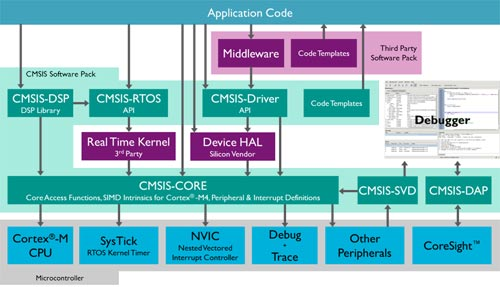
\includegraphics[width=420px, height=280px]{../img/cmsis.jpg}
	\caption{Cortex Microcontroller Software Standard Interface}
	\label{cmsis_}
\end{figure}

\chapter{LWIP}
LwIP is open source TCP/IP protocol suite designed for embedded systems.

The focus of the LwIP TCP/IP implementation is to reduce RAM usage while still
having a full scale TCP. This makes LwIP
suitable for use in embedded systems with tens of kilobytes of free RAM and room
for around 40 kilobytes of code ROM.

LwIP includes the following protocols and features:\citep{lwip-16}

\begin{itemize}
	\item IP (Internet Protocol) including packet forwarding over multiple network interfaces
	\item ICMP (Internet Control Message Protocol) for network maintenance and debugging
	\item IGMP (Internet Group Management Protocol) for multicast traffic management
	\item UDP (User Datagram Protocol) including experimental UDP-lite extensions
	\item TCP (Transmission Control Protocol) with congestion control, RTT estimation and fast recovery/fast retransmit
	\item Raw/native API for enhanced performance
	\item Optional Berkeley-like socket API
	\item DNS (Domain names resolver)
	\item SNMP (Simple Network Management Protocol)
	\item DHCP (Dynamic Host Configuration Protocol)
	\item AUTOIP (for IPv4, conform with RFC 3927)
	\item PPP (Point-to-Point Protocol)
	\item ARP (Address Resolution Protocol) for Ethernet
\end{itemize}




\bibliography{bibliographie}			% Aufruf: bibtex FHWTVorlage
\bibliographystyle{natdin}			% DIN-Stil des Literaturverzeichnisses
% Anhang -------------------------------------------------------------------
%		Die Inhalte des Anhangs werden analog zu den Kapiteln inkludiert.
%		Dies geschieht in der Datei Anhang.tex
% --------------------------------------------------------------------------
% \begin{appendix}
% 	\clearpage
% 	\pagenumbering{roman}
% 	\input{appendix}
% \end{appendix}
\end{document}
